\documentclass[12pt,a4paper]{article}

\usepackage[a4paper,text={16.5cm,25.2cm},centering]{geometry}
\usepackage{lmodern}
\usepackage{amssymb,amsmath}
\usepackage{bm}
\usepackage{graphicx}
\usepackage{microtype}
\usepackage{hyperref}
\setlength{\parindent}{0pt}
\setlength{\parskip}{1.2ex}

\hypersetup
       {   pdfauthor = { Sheehan Olver },
           pdftitle={ foo },
           colorlinks=TRUE,
           linkcolor=black,
           citecolor=blue,
           urlcolor=blue
       }




\usepackage{upquote}
\usepackage{listings}
\usepackage{xcolor}
\lstset{
    basicstyle=\ttfamily\footnotesize,
    upquote=true,
    breaklines=true,
    breakindent=0pt,
    keepspaces=true,
    showspaces=false,
    columns=fullflexible,
    showtabs=false,
    showstringspaces=false,
    escapeinside={(*@}{@*)},
    extendedchars=true,
}
\newcommand{\HLJLt}[1]{#1}
\newcommand{\HLJLw}[1]{#1}
\newcommand{\HLJLe}[1]{#1}
\newcommand{\HLJLeB}[1]{#1}
\newcommand{\HLJLo}[1]{#1}
\newcommand{\HLJLk}[1]{\textcolor[RGB]{148,91,176}{\textbf{#1}}}
\newcommand{\HLJLkc}[1]{\textcolor[RGB]{59,151,46}{\textit{#1}}}
\newcommand{\HLJLkd}[1]{\textcolor[RGB]{214,102,97}{\textit{#1}}}
\newcommand{\HLJLkn}[1]{\textcolor[RGB]{148,91,176}{\textbf{#1}}}
\newcommand{\HLJLkp}[1]{\textcolor[RGB]{148,91,176}{\textbf{#1}}}
\newcommand{\HLJLkr}[1]{\textcolor[RGB]{148,91,176}{\textbf{#1}}}
\newcommand{\HLJLkt}[1]{\textcolor[RGB]{148,91,176}{\textbf{#1}}}
\newcommand{\HLJLn}[1]{#1}
\newcommand{\HLJLna}[1]{#1}
\newcommand{\HLJLnb}[1]{#1}
\newcommand{\HLJLnbp}[1]{#1}
\newcommand{\HLJLnc}[1]{#1}
\newcommand{\HLJLncB}[1]{#1}
\newcommand{\HLJLnd}[1]{\textcolor[RGB]{214,102,97}{#1}}
\newcommand{\HLJLne}[1]{#1}
\newcommand{\HLJLneB}[1]{#1}
\newcommand{\HLJLnf}[1]{\textcolor[RGB]{66,102,213}{#1}}
\newcommand{\HLJLnfm}[1]{\textcolor[RGB]{66,102,213}{#1}}
\newcommand{\HLJLnp}[1]{#1}
\newcommand{\HLJLnl}[1]{#1}
\newcommand{\HLJLnn}[1]{#1}
\newcommand{\HLJLno}[1]{#1}
\newcommand{\HLJLnt}[1]{#1}
\newcommand{\HLJLnv}[1]{#1}
\newcommand{\HLJLnvc}[1]{#1}
\newcommand{\HLJLnvg}[1]{#1}
\newcommand{\HLJLnvi}[1]{#1}
\newcommand{\HLJLnvm}[1]{#1}
\newcommand{\HLJLl}[1]{#1}
\newcommand{\HLJLld}[1]{\textcolor[RGB]{148,91,176}{\textit{#1}}}
\newcommand{\HLJLs}[1]{\textcolor[RGB]{201,61,57}{#1}}
\newcommand{\HLJLsa}[1]{\textcolor[RGB]{201,61,57}{#1}}
\newcommand{\HLJLsb}[1]{\textcolor[RGB]{201,61,57}{#1}}
\newcommand{\HLJLsc}[1]{\textcolor[RGB]{201,61,57}{#1}}
\newcommand{\HLJLsd}[1]{\textcolor[RGB]{201,61,57}{#1}}
\newcommand{\HLJLsdB}[1]{\textcolor[RGB]{201,61,57}{#1}}
\newcommand{\HLJLsdC}[1]{\textcolor[RGB]{201,61,57}{#1}}
\newcommand{\HLJLse}[1]{\textcolor[RGB]{59,151,46}{#1}}
\newcommand{\HLJLsh}[1]{\textcolor[RGB]{201,61,57}{#1}}
\newcommand{\HLJLsi}[1]{#1}
\newcommand{\HLJLso}[1]{\textcolor[RGB]{201,61,57}{#1}}
\newcommand{\HLJLsr}[1]{\textcolor[RGB]{201,61,57}{#1}}
\newcommand{\HLJLss}[1]{\textcolor[RGB]{201,61,57}{#1}}
\newcommand{\HLJLssB}[1]{\textcolor[RGB]{201,61,57}{#1}}
\newcommand{\HLJLnB}[1]{\textcolor[RGB]{59,151,46}{#1}}
\newcommand{\HLJLnbB}[1]{\textcolor[RGB]{59,151,46}{#1}}
\newcommand{\HLJLnfB}[1]{\textcolor[RGB]{59,151,46}{#1}}
\newcommand{\HLJLnh}[1]{\textcolor[RGB]{59,151,46}{#1}}
\newcommand{\HLJLni}[1]{\textcolor[RGB]{59,151,46}{#1}}
\newcommand{\HLJLnil}[1]{\textcolor[RGB]{59,151,46}{#1}}
\newcommand{\HLJLnoB}[1]{\textcolor[RGB]{59,151,46}{#1}}
\newcommand{\HLJLoB}[1]{\textcolor[RGB]{102,102,102}{\textbf{#1}}}
\newcommand{\HLJLow}[1]{\textcolor[RGB]{102,102,102}{\textbf{#1}}}
\newcommand{\HLJLp}[1]{#1}
\newcommand{\HLJLc}[1]{\textcolor[RGB]{153,153,119}{\textit{#1}}}
\newcommand{\HLJLch}[1]{\textcolor[RGB]{153,153,119}{\textit{#1}}}
\newcommand{\HLJLcm}[1]{\textcolor[RGB]{153,153,119}{\textit{#1}}}
\newcommand{\HLJLcp}[1]{\textcolor[RGB]{153,153,119}{\textit{#1}}}
\newcommand{\HLJLcpB}[1]{\textcolor[RGB]{153,153,119}{\textit{#1}}}
\newcommand{\HLJLcs}[1]{\textcolor[RGB]{153,153,119}{\textit{#1}}}
\newcommand{\HLJLcsB}[1]{\textcolor[RGB]{153,153,119}{\textit{#1}}}
\newcommand{\HLJLg}[1]{#1}
\newcommand{\HLJLgd}[1]{#1}
\newcommand{\HLJLge}[1]{#1}
\newcommand{\HLJLgeB}[1]{#1}
\newcommand{\HLJLgh}[1]{#1}
\newcommand{\HLJLgi}[1]{#1}
\newcommand{\HLJLgo}[1]{#1}
\newcommand{\HLJLgp}[1]{#1}
\newcommand{\HLJLgs}[1]{#1}
\newcommand{\HLJLgsB}[1]{#1}
\newcommand{\HLJLgt}[1]{#1}



\def\qqand{\qquad\hbox{and}\qquad}
\def\qqfor{\qquad\hbox{for}\qquad}
\def\D{ {\rm d} }
\def\I{ {\rm i} }
\def\E{ {\rm e} }
\def\C{ {\mathbb C} }
\def\R{ {\mathbb R} }
\def\CC{ {\cal C} }
\def\HH{ {\cal H} }
\def\vc#1{ {\mathbf #1} }
\def\bbC{ {\mathbb C} }

\def\qqqquad{\qquad\qquad}
\def\qqfor{\qquad\hbox{for}\qquad}
\def\qqwhere{\qquad\hbox{where}\qquad}
\def\Res_#1{\underset{#1}{\rm Res}\,}
\def\sech{ {\rm sech}\, }
\def\upepsilon{\varepsilon}


\def\Xint#1{ \mathchoice
   {\XXint\displaystyle\textstyle{#1} }%
   {\XXint\textstyle\scriptstyle{#1} }%
   {\XXint\scriptstyle\scriptscriptstyle{#1} }%
   {\XXint\scriptscriptstyle\scriptscriptstyle{#1} }%
   \!\int}
\def\XXint#1#2#3{ {\setbox0=\hbox{$#1{#2#3}{\int}$}
     \vcenter{\hbox{$#2#3$}}\kern-.5\wd0} }
\def\ddashint{\Xint=}
\def\dashint{\Xint-}
% \def\dashint
\def\infdashint{\dashint_{-\infty}^\infty}




\def\addtab#1={#1\;&=}
\def\ccr{\\\addtab}
\def\ip<#1>{\left\langle{#1}\right\rangle}
\def\dx{\D x}
\def\dt{\D t}
\def\dz{\D z}

\def\norm#1{\left\| #1 \right\|}

\def\pr(#1){\left({#1}\right)}
\def\br[#1]{\left[{#1}\right]}

\def\abs#1{\left|{#1}\right|}
\def\fpr(#1){\!\pr({#1})}

\def\sopmatrix#1{ \begin{pmatrix}#1\end{pmatrix} }

\def\endash{–}
\def\mdblksquare{\blacksquare}
\def\lgblksquare{\blacksquare}
\def\scre{\E}
\def\mapengine#1,#2.{\mapfunction{#1}\ifx\void#2\else\mapengine #2.\fi }

\def\map[#1]{\mapengine #1,\void.}

\def\mapenginesep_#1#2,#3.{\mapfunction{#2}\ifx\void#3\else#1\mapengine #3.\fi }

\def\mapsep_#1[#2]{\mapenginesep_{#1}#2,\void.}


\def\vcbr[#1]{\pr(#1)}


\def\bvect[#1,#2]{
{
\def\dots{\cdots}
\def\mapfunction##1{\ | \  ##1}
	\sopmatrix{
		 \,#1\map[#2]\,
	}
}
}



\def\vect[#1]{
{\def\dots{\ldots}
	\vcbr[{#1}]
} }

\def\vectt[#1]{
{\def\dots{\ldots}
	\vect[{#1}]^{\top}
} }

\def\Vectt[#1]{
{
\def\mapfunction##1{##1 \cr} 
\def\dots{\vdots}
	\begin{pmatrix}
		\map[#1]
	\end{pmatrix}
} }

\def\addtab#1={#1\;&=}
\def\ccr{\\\addtab}

\begin{document}

\textbf{M3M6: Methods of Mathematical Physics}

Dr. Sheehan Olver

s.olver@imperial.ac.uk

\section{Lecture 16: Electrostatic charges in a potential well}
\begin{itemize}
\item[1. ] One charge in a well


\item[2. ] Two charges in a well


\item[3. ] \[
N
\]
charges in a well


\item[4. ] Limiting distribution

\end{itemize}
We study the dynamics of many electric charges in a potential well.  We restrict our attention to 1D:  picture an infinitely long wire with carges on it. We will see that as the number of charges becomes large,  we can determine the limiting distribution by inverting the Hilbert transform, but one which the \emph{interval}  its posed on is solved for.

\subsection{One charge in a potential well}
Consider a point charge in a well $V(x) = x^2 / 2$, initially located at $\lambda^0$.  The dynamics of the point charge are governed by Newton's law

\[
m { \D \lambda^2 \over \dt^2} + \gamma { \D \lambda \over \dt}  = -V'(\lambda) = -  \lambda
\]
Here $m$ is the mass (we will always take it to be 1) and $\gamma$ is a damping constant (think friction) which ensures that the charge eventially comes to  rest. 

This is a simple damped harmonic oscillator: if we are positive we move left and if we are negative we move right.  Here we show the evolution as a function of time, where we plot this on top of the potential to see its effect.


\begin{lstlisting}
(*@\HLJLk{using}@*) (*@\HLJLn{DifferentialEquations}@*)(*@\HLJLp{,}@*) (*@\HLJLn{Plots}@*)(*@\HLJLp{,}@*) (*@\HLJLn{StaticArrays}@*)
(*@\HLJLn{V}@*) (*@\HLJLoB{=}@*) (*@\HLJLn{x}@*) (*@\HLJLoB{->}@*) (*@\HLJLn{x}@*)(*@\HLJLoB{{\textasciicircum}}@*)(*@\HLJLni{2}@*)(*@\HLJLoB{/}@*)(*@\HLJLni{2}@*)  (*@\HLJLcs{{\#}}@*) (*@\HLJLcs{Potential}@*)
(*@\HLJLn{Vp}@*) (*@\HLJLoB{=}@*) (*@\HLJLn{x}@*) (*@\HLJLoB{->}@*) (*@\HLJLn{x}@*)     (*@\HLJLcs{{\#}}@*) (*@\HLJLcs{Force}@*)

(*@\HLJLn{\ensuremath{\lambda}{\_}0}@*) (*@\HLJLoB{=}@*) (*@\HLJLnfB{2.3}@*)  (*@\HLJLcs{{\#}}@*) (*@\HLJLcs{initial}@*) (*@\HLJLcs{location}@*)
(*@\HLJLn{v{\_}0}@*) (*@\HLJLoB{=}@*) (*@\HLJLnfB{1.2}@*)  (*@\HLJLcs{{\#}}@*) (*@\HLJLcs{initial}@*) (*@\HLJLcs{position}@*)
(*@\HLJLn{\ensuremath{\gamma}}@*) (*@\HLJLoB{=}@*) (*@\HLJLnfB{1.0}@*)    (*@\HLJLcs{{\#}}@*) (*@\HLJLcs{damping}@*)

(*@\HLJLn{\ensuremath{\lambda}v}@*) (*@\HLJLoB{=}@*) (*@\HLJLnf{solve}@*)(*@\HLJLp{(}@*)(*@\HLJLnf{ODEProblem}@*)(*@\HLJLp{(((}@*)(*@\HLJLn{\ensuremath{\lambda}}@*)(*@\HLJLp{,}@*)(*@\HLJLn{v}@*)(*@\HLJLp{),}@*)(*@\HLJLn{{\_}}@*)(*@\HLJLp{,}@*)(*@\HLJLn{t}@*)(*@\HLJLp{)}@*) (*@\HLJLoB{->}@*) (*@\HLJLnf{SVector}@*)(*@\HLJLp{(}@*)(*@\HLJLn{v}@*)(*@\HLJLp{,}@*)(*@\HLJLoB{-}@*)(*@\HLJLnf{Vp}@*)(*@\HLJLp{(}@*)(*@\HLJLn{\ensuremath{\lambda}}@*)(*@\HLJLp{)}@*) (*@\HLJLoB{-}@*) (*@\HLJLn{\ensuremath{\gamma}}@*)(*@\HLJLoB{*}@*)(*@\HLJLn{v}@*)(*@\HLJLp{),}@*) (*@\HLJLnf{SVector}@*)(*@\HLJLp{(}@*)(*@\HLJLn{\ensuremath{\lambda}{\_}0}@*)(*@\HLJLp{,}@*)(*@\HLJLn{v{\_}0}@*)(*@\HLJLp{),}@*) (*@\HLJLp{(}@*)(*@\HLJLnfB{0.0}@*)(*@\HLJLp{,}@*) (*@\HLJLnfB{20.0}@*)(*@\HLJLp{));}@*) (*@\HLJLn{reltol}@*)(*@\HLJLoB{=}@*)(*@\HLJLnfB{1E-6}@*)(*@\HLJLp{);}@*)

(*@\HLJLn{tt}@*) (*@\HLJLoB{=}@*) (*@\HLJLnf{range}@*)(*@\HLJLp{(}@*)(*@\HLJLnfB{0.}@*)(*@\HLJLp{,}@*)(*@\HLJLni{20}@*)(*@\HLJLp{;}@*) (*@\HLJLn{length}@*)(*@\HLJLoB{=}@*)(*@\HLJLni{1000}@*)(*@\HLJLp{)}@*)
(*@\HLJLn{xx}@*) (*@\HLJLoB{=}@*) (*@\HLJLnf{range}@*)(*@\HLJLp{(}@*)(*@\HLJLoB{-}@*)(*@\HLJLnf{sqrt}@*)(*@\HLJLp{(}@*)(*@\HLJLni{2}@*)(*@\HLJLoB{*}@*)(*@\HLJLnf{last}@*)(*@\HLJLp{(}@*)(*@\HLJLn{tt}@*)(*@\HLJLp{)),}@*)(*@\HLJLnf{sqrt}@*)(*@\HLJLp{(}@*)(*@\HLJLni{2}@*)(*@\HLJLoB{*}@*)(*@\HLJLnf{last}@*)(*@\HLJLp{(}@*)(*@\HLJLn{tt}@*)(*@\HLJLp{));}@*) (*@\HLJLn{length}@*)(*@\HLJLoB{=}@*)(*@\HLJLni{1000}@*)(*@\HLJLp{)}@*)
(*@\HLJLnf{plot}@*)(*@\HLJLp{(}@*)(*@\HLJLn{xx}@*)(*@\HLJLp{,}@*) (*@\HLJLn{V}@*)(*@\HLJLoB{.}@*)(*@\HLJLp{(}@*)(*@\HLJLn{xx}@*)(*@\HLJLp{);}@*) (*@\HLJLn{label}@*)(*@\HLJLoB{=}@*)(*@\HLJLs{"{}potential"{}}@*)(*@\HLJLp{,}@*) (*@\HLJLn{xlabel}@*)(*@\HLJLoB{=}@*)(*@\HLJLs{"{}x"{}}@*)(*@\HLJLp{,}@*) (*@\HLJLn{ylabel}@*)(*@\HLJLoB{=}@*)(*@\HLJLs{"{}time}@*) (*@\HLJLs{and}@*) (*@\HLJLs{potential"{}}@*)(*@\HLJLp{)}@*)
(*@\HLJLnf{plot!}@*)(*@\HLJLp{(}@*)(*@\HLJLn{first}@*)(*@\HLJLoB{.}@*)(*@\HLJLp{(}@*)(*@\HLJLn{\ensuremath{\lambda}v}@*)(*@\HLJLoB{.}@*)(*@\HLJLp{(}@*)(*@\HLJLn{tt}@*)(*@\HLJLp{)),}@*) (*@\HLJLn{tt}@*)(*@\HLJLp{;}@*) (*@\HLJLn{label}@*)(*@\HLJLoB{=}@*)(*@\HLJLs{"{}charge"{}}@*)(*@\HLJLp{)}@*)
\end{lstlisting}

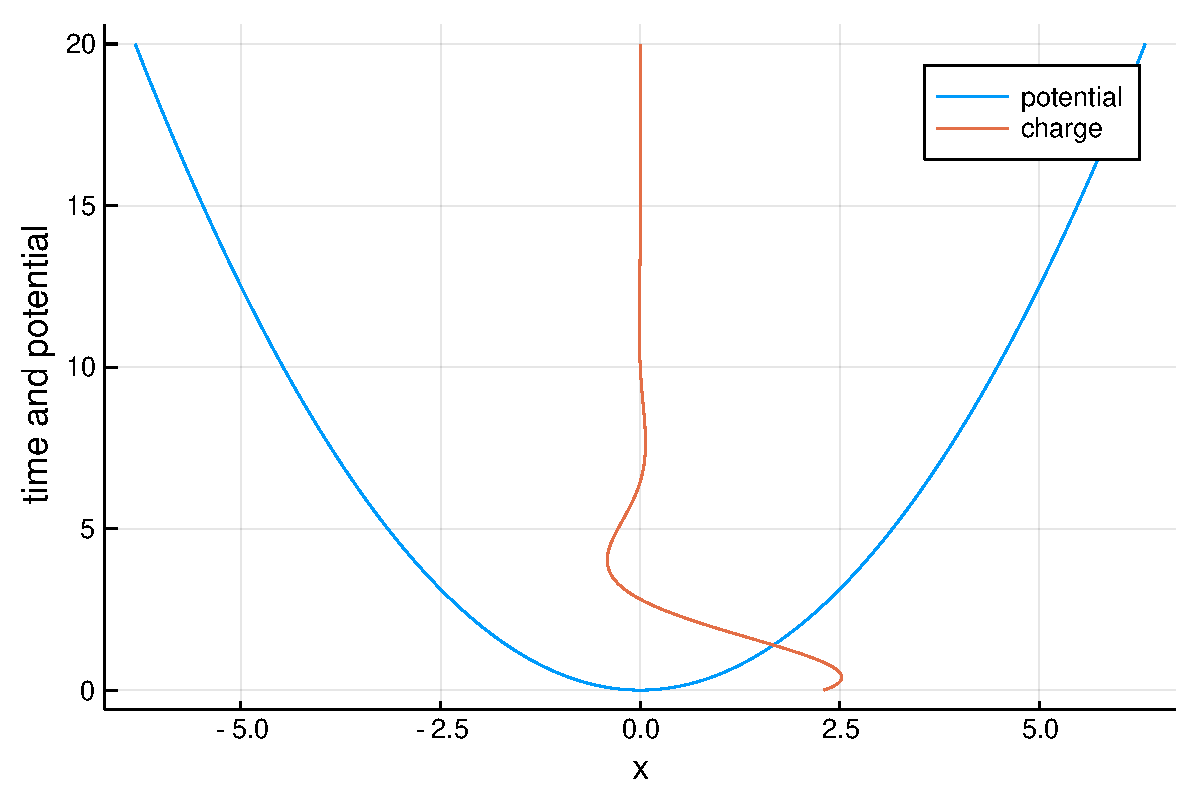
\includegraphics[width=\linewidth]{figures/Lecture16_1_1.pdf}

In the limit the charge reaches an equilibrium: it no longer varies in time. I.e.,  it reaches a point where ${ \D \lambda^2 \over \dt^2} = { \D \lambda \over \dt}  = 0$, which is equivalent to solving

\[
 0 = - V'(\lambda)  = - \lambda
\]
in other words, the minimum of the well, in this case $\lambda = 0$.

\subsection{Two charges in a potential well}
A point charge at $x_0$ in 2D creates a (Newtonian) potential field of $V_{x_0}(x) = -\log|x - x_0|$ with derivative

\[
V_{x_0}'(x) = \begin{cases} -{1 \over x - x_0} & x > x_0 \\
        {1 \over x_0 - x} & x < x_0 
\end{cases} = {1 \over x_0 - x}
\]
Here we are thinking of the charges as 2D but restricted to the real line: think of a 1D wire embedded in 2D space. 

Suppose there are now two charges, $\lambda_1$ and $\lambda_2$ but no potential well.  The effect on the first charge $\lambda_1$ is  to repulse away from $\lambda_2$ via the potential field $V_{\lambda_2}(x) = -\log|x - \lambda_2|$. Since we have

\[
m {\D^2 \lambda_1 \over \D t^2} = - V_{\lambda_2}'(\lambda_1) =  {1 \over \lambda_1 -\lambda_2}
\]
Similarly, the effect on $\lambda_2$ is

\[
m {\D^2 \lambda_2 \over \D t^2} = {1 \over \lambda_2 -\lambda_1}
\]
Unrestricted, the two potentials will repulse off to infinity:


\begin{lstlisting}
(*@\HLJLn{N}@*) (*@\HLJLoB{=}@*) (*@\HLJLni{2}@*)
(*@\HLJLn{\ensuremath{\lambda}{\_}0}@*) (*@\HLJLoB{=}@*) (*@\HLJLnf{randn}@*)(*@\HLJLp{(}@*)(*@\HLJLni{2}@*)(*@\HLJLp{)}@*)  (*@\HLJLcs{{\#}}@*) (*@\HLJLcs{random}@*) (*@\HLJLcs{initial}@*) (*@\HLJLcs{location}@*)
(*@\HLJLn{v{\_}0}@*) (*@\HLJLoB{=}@*) (*@\HLJLnf{randn}@*)(*@\HLJLp{(}@*)(*@\HLJLni{2}@*)(*@\HLJLp{)}@*)  (*@\HLJLcs{{\#}}@*) (*@\HLJLcs{random}@*) (*@\HLJLcs{initial}@*) (*@\HLJLcs{velocity}@*)
(*@\HLJLn{prob}@*) (*@\HLJLoB{=}@*) (*@\HLJLnf{ODEProblem}@*)(*@\HLJLp{(}@*)(*@\HLJLk{function}@*)(*@\HLJLp{(}@*)(*@\HLJLn{\ensuremath{\lambda}v}@*)(*@\HLJLp{,}@*)(*@\HLJLn{{\_}}@*)(*@\HLJLp{,}@*)(*@\HLJLn{t}@*)(*@\HLJLp{)}@*) 
        (*@\HLJLn{\ensuremath{\lambda}}@*) (*@\HLJLoB{=}@*) (*@\HLJLn{\ensuremath{\lambda}v}@*)(*@\HLJLp{[}@*)(*@\HLJLni{1}@*)(*@\HLJLoB{:}@*)(*@\HLJLn{N}@*)(*@\HLJLp{]}@*)
        (*@\HLJLn{v}@*) (*@\HLJLoB{=}@*) (*@\HLJLn{\ensuremath{\lambda}v}@*)(*@\HLJLp{[}@*)(*@\HLJLn{N}@*)(*@\HLJLoB{+}@*)(*@\HLJLni{1}@*)(*@\HLJLoB{:}@*)(*@\HLJLk{end}@*)(*@\HLJLp{]}@*)
        (*@\HLJLp{[}@*)(*@\HLJLn{v}@*)(*@\HLJLp{;}@*) (*@\HLJLni{1}@*)(*@\HLJLoB{/}@*)(*@\HLJLp{(}@*)(*@\HLJLn{\ensuremath{\lambda}}@*)(*@\HLJLp{[}@*)(*@\HLJLni{1}@*)(*@\HLJLp{]}@*) (*@\HLJLoB{-}@*) (*@\HLJLn{\ensuremath{\lambda}}@*)(*@\HLJLp{[}@*)(*@\HLJLni{2}@*)(*@\HLJLp{]);}@*) (*@\HLJLni{1}@*)(*@\HLJLoB{/}@*)(*@\HLJLp{(}@*)(*@\HLJLn{\ensuremath{\lambda}}@*)(*@\HLJLp{[}@*)(*@\HLJLni{2}@*)(*@\HLJLp{]}@*) (*@\HLJLoB{-}@*) (*@\HLJLn{\ensuremath{\lambda}}@*)(*@\HLJLp{[}@*)(*@\HLJLni{1}@*)(*@\HLJLp{])]}@*)
        (*@\HLJLk{end}@*)(*@\HLJLp{,}@*) (*@\HLJLp{[}@*)(*@\HLJLn{\ensuremath{\lambda}{\_}0}@*)(*@\HLJLp{;}@*) (*@\HLJLn{v{\_}0}@*)(*@\HLJLp{],}@*) (*@\HLJLp{(}@*)(*@\HLJLnfB{0.0}@*)(*@\HLJLp{,}@*) (*@\HLJLnfB{10.0}@*)(*@\HLJLp{))}@*)
(*@\HLJLn{\ensuremath{\lambda}v}@*) (*@\HLJLoB{=}@*) (*@\HLJLnf{solve}@*)(*@\HLJLp{(}@*)(*@\HLJLn{prob}@*)(*@\HLJLp{;}@*) (*@\HLJLn{reltol}@*)(*@\HLJLoB{=}@*)(*@\HLJLnfB{1E-6}@*)(*@\HLJLp{)}@*)
(*@\HLJLn{tt}@*) (*@\HLJLoB{=}@*) (*@\HLJLnf{range}@*)(*@\HLJLp{(}@*)(*@\HLJLnfB{0.}@*)(*@\HLJLp{,}@*)(*@\HLJLni{20}@*)(*@\HLJLp{;}@*) (*@\HLJLn{length}@*)(*@\HLJLoB{=}@*)(*@\HLJLni{1000}@*)(*@\HLJLp{)}@*)
(*@\HLJLnf{\ensuremath{\lambda}v}@*)(*@\HLJLp{(}@*)(*@\HLJLnfB{0.1}@*)(*@\HLJLp{)}@*)

(*@\HLJLn{p}@*) (*@\HLJLoB{=}@*) (*@\HLJLnf{plot}@*)(*@\HLJLp{(;}@*)(*@\HLJLn{xlabel}@*)(*@\HLJLoB{=}@*)(*@\HLJLs{"{}x"{}}@*)(*@\HLJLp{,}@*)(*@\HLJLn{ylabel}@*)(*@\HLJLoB{=}@*)(*@\HLJLs{"{}t"{}}@*)(*@\HLJLp{)}@*)
(*@\HLJLk{for}@*) (*@\HLJLn{j}@*) (*@\HLJLoB{=}@*) (*@\HLJLni{1}@*)(*@\HLJLoB{:}@*)(*@\HLJLn{N}@*)
    (*@\HLJLnf{plot!}@*)(*@\HLJLp{(}@*)(*@\HLJLn{getindex}@*)(*@\HLJLoB{.}@*)(*@\HLJLp{(}@*)(*@\HLJLn{\ensuremath{\lambda}v}@*)(*@\HLJLoB{.}@*)(*@\HLJLp{(}@*)(*@\HLJLn{tt}@*)(*@\HLJLp{),}@*)(*@\HLJLn{j}@*)(*@\HLJLp{),}@*) (*@\HLJLn{tt}@*)(*@\HLJLp{;}@*) (*@\HLJLn{label}@*)(*@\HLJLoB{=}@*)(*@\HLJLs{"{}charge}@*) (*@\HLJLsi{{\$}j}@*)(*@\HLJLs{"{}}@*)(*@\HLJLp{)}@*)
(*@\HLJLk{end}@*)
(*@\HLJLn{p}@*)
\end{lstlisting}

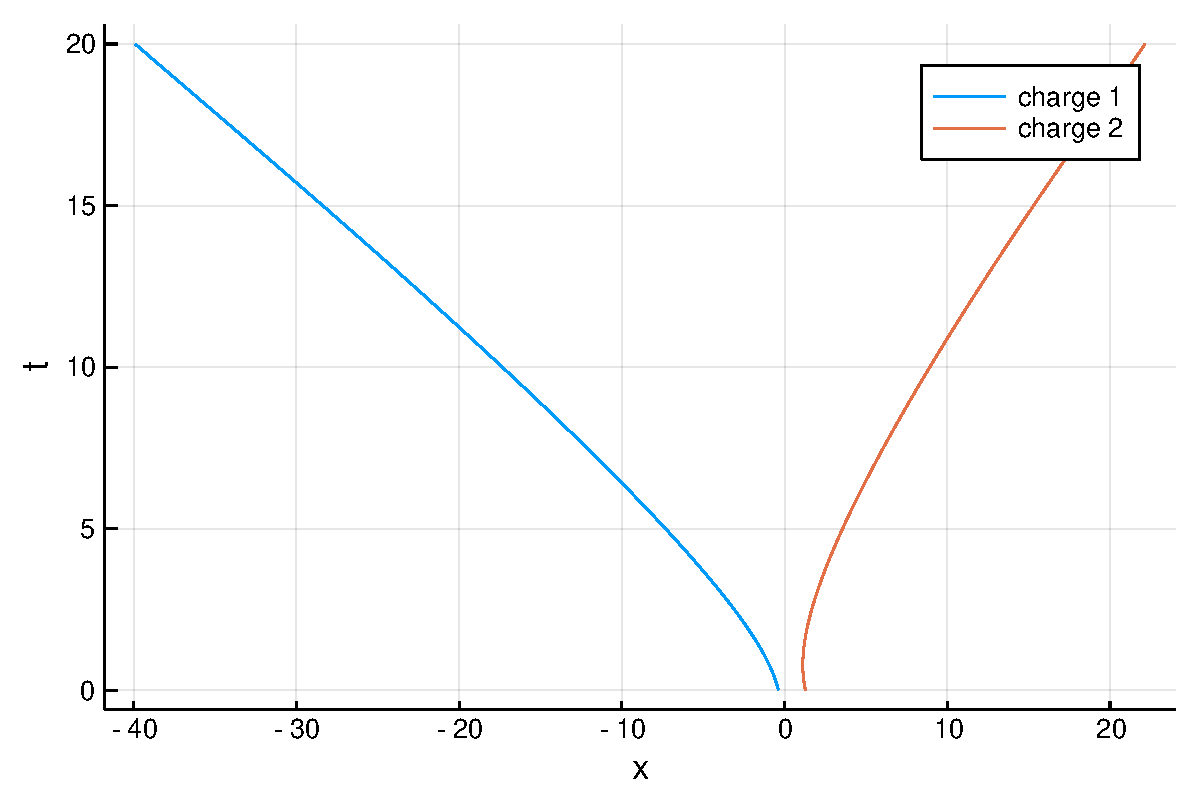
\includegraphics[width=\linewidth]{figures/Lecture16_2_1.pdf}

Adding in a potential well and damping and we get an equilbrium again:


\begin{align*}
{\D^2 \lambda_1 \over \D t^2} + \gamma {\D \lambda_1 \over \dt} = {1 \over \lambda_1 -\lambda_2} - V'(\lambda_1) \\
{\D^2 \lambda_2 \over \D t^2}+ \gamma {\D \lambda_2 \over \dt} = {1 \over \lambda_2 -\lambda_1} - V'(\lambda_2)
\end{align*}
which we see here


\begin{lstlisting}
(*@\HLJLn{V}@*) (*@\HLJLoB{=}@*) (*@\HLJLn{x}@*) (*@\HLJLoB{->}@*) (*@\HLJLn{x}@*)(*@\HLJLoB{{\textasciicircum}}@*)(*@\HLJLni{2}@*)(*@\HLJLoB{/}@*)(*@\HLJLni{2}@*)  (*@\HLJLcs{{\#}}@*) (*@\HLJLcs{Potential}@*)
(*@\HLJLn{Vp}@*) (*@\HLJLoB{=}@*) (*@\HLJLn{x}@*) (*@\HLJLoB{->}@*) (*@\HLJLn{x}@*)     (*@\HLJLcs{{\#}}@*) (*@\HLJLcs{Force}@*)
(*@\HLJLn{\ensuremath{\gamma}}@*) (*@\HLJLoB{=}@*) (*@\HLJLnfB{1.0}@*)    (*@\HLJLcs{{\#}}@*) (*@\HLJLcs{damping}@*)

(*@\HLJLn{prob}@*) (*@\HLJLoB{=}@*) (*@\HLJLnf{ODEProblem}@*)(*@\HLJLp{(}@*)(*@\HLJLk{function}@*)(*@\HLJLp{(}@*)(*@\HLJLn{\ensuremath{\lambda}v}@*)(*@\HLJLp{,}@*)(*@\HLJLn{{\_}}@*)(*@\HLJLp{,}@*)(*@\HLJLn{t}@*)(*@\HLJLp{)}@*) 
        (*@\HLJLn{\ensuremath{\lambda}}@*) (*@\HLJLoB{=}@*) (*@\HLJLn{\ensuremath{\lambda}v}@*)(*@\HLJLp{[}@*)(*@\HLJLni{1}@*)(*@\HLJLoB{:}@*)(*@\HLJLn{N}@*)(*@\HLJLp{]}@*)
        (*@\HLJLn{v}@*) (*@\HLJLoB{=}@*) (*@\HLJLn{\ensuremath{\lambda}v}@*)(*@\HLJLp{[}@*)(*@\HLJLn{N}@*)(*@\HLJLoB{+}@*)(*@\HLJLni{1}@*)(*@\HLJLoB{:}@*)(*@\HLJLk{end}@*)(*@\HLJLp{]}@*)
        (*@\HLJLp{[}@*)(*@\HLJLn{v}@*)(*@\HLJLp{;}@*) (*@\HLJLni{1}@*)(*@\HLJLoB{/}@*)(*@\HLJLp{(}@*)(*@\HLJLn{\ensuremath{\lambda}}@*)(*@\HLJLp{[}@*)(*@\HLJLni{1}@*)(*@\HLJLp{]}@*) (*@\HLJLoB{-}@*) (*@\HLJLn{\ensuremath{\lambda}}@*)(*@\HLJLp{[}@*)(*@\HLJLni{2}@*)(*@\HLJLp{])}@*) (*@\HLJLoB{-}@*) (*@\HLJLnf{Vp}@*)(*@\HLJLp{(}@*)(*@\HLJLn{\ensuremath{\lambda}}@*)(*@\HLJLp{[}@*)(*@\HLJLni{1}@*)(*@\HLJLp{])}@*) (*@\HLJLoB{-}@*) (*@\HLJLn{\ensuremath{\gamma}}@*)(*@\HLJLoB{*}@*)(*@\HLJLn{v}@*)(*@\HLJLp{[}@*)(*@\HLJLni{1}@*)(*@\HLJLp{];}@*) (*@\HLJLni{1}@*)(*@\HLJLoB{/}@*)(*@\HLJLp{(}@*)(*@\HLJLn{\ensuremath{\lambda}}@*)(*@\HLJLp{[}@*)(*@\HLJLni{2}@*)(*@\HLJLp{]}@*) (*@\HLJLoB{-}@*) (*@\HLJLn{\ensuremath{\lambda}}@*)(*@\HLJLp{[}@*)(*@\HLJLni{1}@*)(*@\HLJLp{])}@*)  (*@\HLJLoB{-}@*) (*@\HLJLnf{Vp}@*)(*@\HLJLp{(}@*)(*@\HLJLn{\ensuremath{\lambda}}@*)(*@\HLJLp{[}@*)(*@\HLJLni{2}@*)(*@\HLJLp{])}@*) (*@\HLJLoB{-}@*) (*@\HLJLn{\ensuremath{\gamma}}@*)(*@\HLJLoB{*}@*)(*@\HLJLn{v}@*)(*@\HLJLp{[}@*)(*@\HLJLni{2}@*)(*@\HLJLp{]]}@*)
        (*@\HLJLk{end}@*)(*@\HLJLp{,}@*) (*@\HLJLp{[}@*)(*@\HLJLn{\ensuremath{\lambda}{\_}0}@*)(*@\HLJLp{;}@*) (*@\HLJLn{v{\_}0}@*)(*@\HLJLp{],}@*) (*@\HLJLp{(}@*)(*@\HLJLnfB{0.0}@*)(*@\HLJLp{,}@*) (*@\HLJLnfB{20.0}@*)(*@\HLJLp{))}@*)
(*@\HLJLn{\ensuremath{\lambda}v}@*) (*@\HLJLoB{=}@*) (*@\HLJLnf{solve}@*)(*@\HLJLp{(}@*)(*@\HLJLn{prob}@*)(*@\HLJLp{;}@*) (*@\HLJLn{reltol}@*)(*@\HLJLoB{=}@*)(*@\HLJLnfB{1E-6}@*)(*@\HLJLp{);}@*)

(*@\HLJLn{xx}@*) (*@\HLJLoB{=}@*) (*@\HLJLnf{range}@*)(*@\HLJLp{(}@*)(*@\HLJLoB{-}@*)(*@\HLJLnf{sqrt}@*)(*@\HLJLp{(}@*)(*@\HLJLni{2}@*)(*@\HLJLoB{*}@*)(*@\HLJLnf{last}@*)(*@\HLJLp{(}@*)(*@\HLJLn{tt}@*)(*@\HLJLp{)),}@*)(*@\HLJLnf{sqrt}@*)(*@\HLJLp{(}@*)(*@\HLJLni{2}@*)(*@\HLJLoB{*}@*)(*@\HLJLnf{last}@*)(*@\HLJLp{(}@*)(*@\HLJLn{tt}@*)(*@\HLJLp{));}@*) (*@\HLJLn{length}@*)(*@\HLJLoB{=}@*)(*@\HLJLni{1000}@*)(*@\HLJLp{)}@*)
(*@\HLJLn{p}@*) (*@\HLJLoB{=}@*) (*@\HLJLnf{plot}@*)(*@\HLJLp{(}@*)(*@\HLJLn{xx}@*)(*@\HLJLp{,}@*) (*@\HLJLn{V}@*)(*@\HLJLoB{.}@*)(*@\HLJLp{(}@*)(*@\HLJLn{xx}@*)(*@\HLJLp{);}@*) (*@\HLJLn{label}@*)(*@\HLJLoB{=}@*)(*@\HLJLs{"{}potential"{}}@*)(*@\HLJLp{,}@*) (*@\HLJLn{xlabel}@*)(*@\HLJLoB{=}@*)(*@\HLJLs{"{}x"{}}@*)(*@\HLJLp{,}@*) (*@\HLJLn{ylabel}@*)(*@\HLJLoB{=}@*)(*@\HLJLs{"{}time}@*) (*@\HLJLs{and}@*) (*@\HLJLs{potential"{}}@*)(*@\HLJLp{)}@*)
(*@\HLJLk{for}@*) (*@\HLJLn{j}@*) (*@\HLJLoB{=}@*) (*@\HLJLni{1}@*)(*@\HLJLoB{:}@*)(*@\HLJLn{N}@*)
    (*@\HLJLnf{plot!}@*)(*@\HLJLp{(}@*)(*@\HLJLn{getindex}@*)(*@\HLJLoB{.}@*)(*@\HLJLp{(}@*)(*@\HLJLn{\ensuremath{\lambda}v}@*)(*@\HLJLoB{.}@*)(*@\HLJLp{(}@*)(*@\HLJLn{tt}@*)(*@\HLJLp{),}@*)(*@\HLJLn{j}@*)(*@\HLJLp{),}@*) (*@\HLJLn{tt}@*)(*@\HLJLp{;}@*) (*@\HLJLn{label}@*)(*@\HLJLoB{=}@*)(*@\HLJLs{"{}charge}@*) (*@\HLJLsi{{\$}j}@*)(*@\HLJLs{"{}}@*)(*@\HLJLp{)}@*)
(*@\HLJLk{end}@*)
(*@\HLJLn{p}@*)
\end{lstlisting}

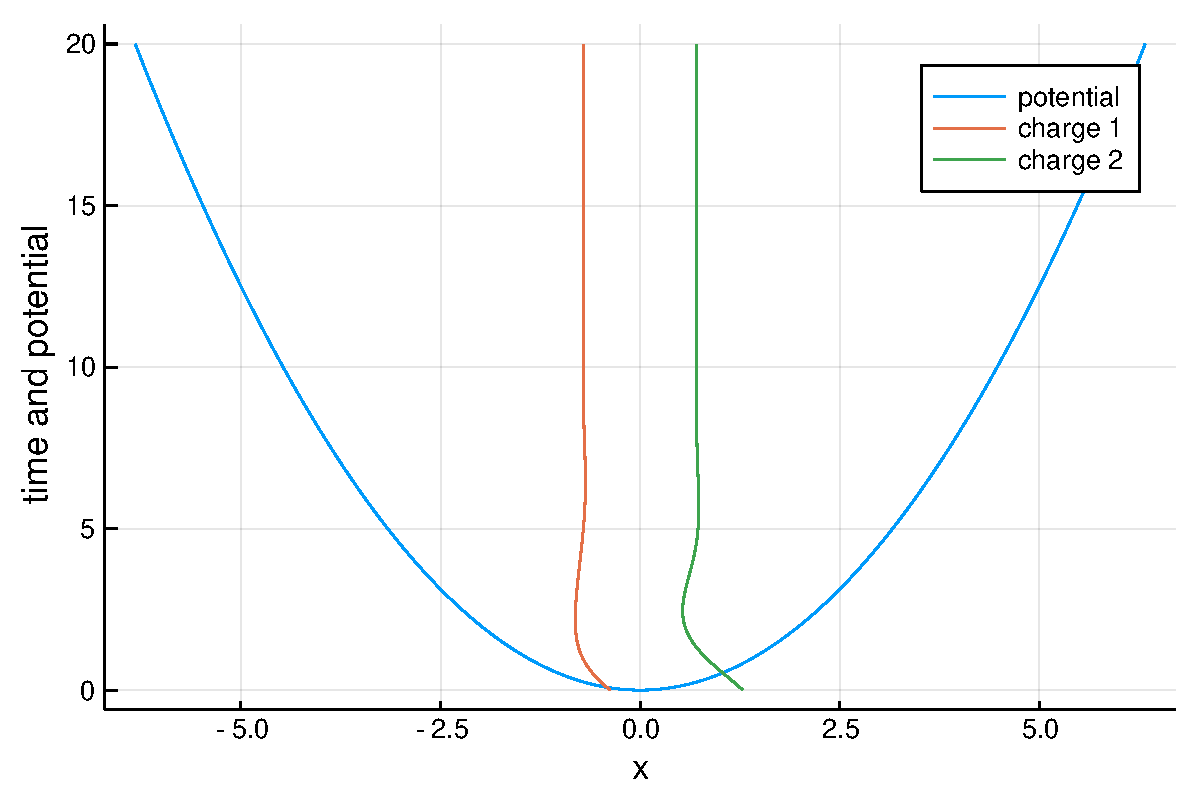
\includegraphics[width=\linewidth]{figures/Lecture16_3_1.pdf}

The fixed point is when the change with time vanishes, given by


\begin{align*}
0 = {1 \over \lambda_1 -\lambda_2} - V'(\lambda_1) \\
0 = {1 \over \lambda_2 -\lambda_1} - V'(\lambda_2) 
\end{align*}
For this potential, we can solve it exactly: we need to solve


\begin{align*}
\lambda_1 = {1 \over \lambda_1 -\lambda_2}  \\
\lambda_2 = {1 \over \lambda_2 -\lambda_1} 
\end{align*}
Using $\lambda_1 = -\lambda_2$, we find that $\lambda_1 = \pm{1 \over \sqrt 2}$.

\subsubsection{$N$ charges in a potential well}
We now consider $N$ charges, where each charge repulses every other charge by a logarithmic potential,  so we end up needing to sum over them all others:


\begin{align*}
m {\D^2 \lambda_k \over \D t^2} + \gamma {\D \lambda_k \over \dt}  = 
    \sum_{j=1 \atop j \neq k}^N {1 \over \lambda_k -\lambda_j} - V'(\lambda_k) 
\end{align*}

\begin{lstlisting}
(*@\HLJLn{N}@*) (*@\HLJLoB{=}@*) (*@\HLJLni{100}@*)

(*@\HLJLn{V}@*) (*@\HLJLoB{=}@*) (*@\HLJLn{x}@*) (*@\HLJLoB{->}@*) (*@\HLJLn{x}@*)(*@\HLJLoB{{\textasciicircum}}@*)(*@\HLJLni{2}@*)(*@\HLJLoB{/}@*)(*@\HLJLni{2}@*)  (*@\HLJLcs{{\#}}@*) (*@\HLJLcs{Potential}@*)
(*@\HLJLn{Vp}@*) (*@\HLJLoB{=}@*) (*@\HLJLn{x}@*) (*@\HLJLoB{->}@*) (*@\HLJLn{x}@*)     (*@\HLJLcs{{\#}}@*) (*@\HLJLcs{Force}@*)

(*@\HLJLn{\ensuremath{\lambda}{\_}0}@*) (*@\HLJLoB{=}@*) (*@\HLJLnf{randn}@*)(*@\HLJLp{(}@*)(*@\HLJLn{N}@*)(*@\HLJLp{)}@*)  (*@\HLJLcs{{\#}}@*) (*@\HLJLcs{initial}@*) (*@\HLJLcs{location}@*)
(*@\HLJLn{v{\_}0}@*) (*@\HLJLoB{=}@*) (*@\HLJLnf{randn}@*)(*@\HLJLp{(}@*)(*@\HLJLn{N}@*)(*@\HLJLp{)}@*)  (*@\HLJLcs{{\#}}@*) (*@\HLJLcs{initial}@*) (*@\HLJLcs{velocity}@*)
(*@\HLJLn{\ensuremath{\gamma}}@*) (*@\HLJLoB{=}@*) (*@\HLJLnfB{1.0}@*)    (*@\HLJLcs{{\#}}@*) (*@\HLJLcs{damping}@*)

(*@\HLJLn{prob}@*) (*@\HLJLoB{=}@*) (*@\HLJLnf{ODEProblem}@*)(*@\HLJLp{(}@*)(*@\HLJLk{function}@*)(*@\HLJLp{(}@*)(*@\HLJLn{\ensuremath{\lambda}v}@*)(*@\HLJLp{,}@*)(*@\HLJLn{{\_}}@*)(*@\HLJLp{,}@*)(*@\HLJLn{t}@*)(*@\HLJLp{)}@*) 
        (*@\HLJLn{\ensuremath{\lambda}}@*) (*@\HLJLoB{=}@*) (*@\HLJLn{\ensuremath{\lambda}v}@*)(*@\HLJLp{[}@*)(*@\HLJLni{1}@*)(*@\HLJLoB{:}@*)(*@\HLJLn{N}@*)(*@\HLJLp{]}@*)
        (*@\HLJLn{v}@*) (*@\HLJLoB{=}@*) (*@\HLJLn{\ensuremath{\lambda}v}@*)(*@\HLJLp{[}@*)(*@\HLJLn{N}@*)(*@\HLJLoB{+}@*)(*@\HLJLni{1}@*)(*@\HLJLoB{:}@*)(*@\HLJLk{end}@*)(*@\HLJLp{]}@*)
        (*@\HLJLp{[}@*)(*@\HLJLn{v}@*)(*@\HLJLp{;}@*) (*@\HLJLp{[}@*)(*@\HLJLnf{sum}@*)(*@\HLJLp{(}@*)(*@\HLJLni{1}@*) (*@\HLJLoB{./}@*) (*@\HLJLp{(}@*)(*@\HLJLn{\ensuremath{\lambda}}@*)(*@\HLJLp{[}@*)(*@\HLJLn{k}@*)(*@\HLJLp{]}@*) (*@\HLJLoB{.-}@*) (*@\HLJLn{\ensuremath{\lambda}}@*)(*@\HLJLp{[[}@*)(*@\HLJLni{1}@*)(*@\HLJLoB{:}@*)(*@\HLJLn{k}@*)(*@\HLJLoB{-}@*)(*@\HLJLni{1}@*)(*@\HLJLp{;}@*)(*@\HLJLn{k}@*)(*@\HLJLoB{+}@*)(*@\HLJLni{1}@*)(*@\HLJLoB{:}@*)(*@\HLJLk{end}@*)(*@\HLJLp{]]))}@*) (*@\HLJLoB{-}@*) (*@\HLJLnf{Vp}@*)(*@\HLJLp{(}@*)(*@\HLJLn{\ensuremath{\lambda}}@*)(*@\HLJLp{[}@*)(*@\HLJLn{k}@*)(*@\HLJLp{])}@*) (*@\HLJLoB{-}@*)  (*@\HLJLn{\ensuremath{\gamma}}@*)(*@\HLJLoB{*}@*)(*@\HLJLn{v}@*)(*@\HLJLp{[}@*)(*@\HLJLn{k}@*)(*@\HLJLp{]}@*) (*@\HLJLk{for}@*) (*@\HLJLn{k}@*)(*@\HLJLoB{=}@*)(*@\HLJLni{1}@*)(*@\HLJLoB{:}@*)(*@\HLJLn{N}@*)(*@\HLJLp{]]}@*)
        (*@\HLJLk{end}@*)(*@\HLJLp{,}@*) (*@\HLJLp{[}@*)(*@\HLJLn{\ensuremath{\lambda}{\_}0}@*)(*@\HLJLp{;}@*) (*@\HLJLn{v{\_}0}@*)(*@\HLJLp{],}@*) (*@\HLJLp{(}@*)(*@\HLJLnfB{0.0}@*)(*@\HLJLp{,}@*) (*@\HLJLnfB{20.0}@*)(*@\HLJLp{))}@*)
(*@\HLJLn{\ensuremath{\lambda}v}@*) (*@\HLJLoB{=}@*) (*@\HLJLnf{solve}@*)(*@\HLJLp{(}@*)(*@\HLJLn{prob}@*)(*@\HLJLp{;}@*) (*@\HLJLn{reltol}@*)(*@\HLJLoB{=}@*)(*@\HLJLnfB{1E-6}@*)(*@\HLJLp{)}@*)

(*@\HLJLn{xx}@*) (*@\HLJLoB{=}@*) (*@\HLJLnf{range}@*)(*@\HLJLp{(}@*)(*@\HLJLoB{-}@*)(*@\HLJLnf{sqrt}@*)(*@\HLJLp{(}@*)(*@\HLJLni{2}@*)(*@\HLJLoB{*}@*)(*@\HLJLnf{last}@*)(*@\HLJLp{(}@*)(*@\HLJLn{tt}@*)(*@\HLJLp{)),}@*)(*@\HLJLnf{sqrt}@*)(*@\HLJLp{(}@*)(*@\HLJLni{2}@*)(*@\HLJLoB{*}@*)(*@\HLJLnf{last}@*)(*@\HLJLp{(}@*)(*@\HLJLn{tt}@*)(*@\HLJLp{));}@*) (*@\HLJLn{length}@*)(*@\HLJLoB{=}@*)(*@\HLJLni{1000}@*)(*@\HLJLp{)}@*)
(*@\HLJLn{p}@*) (*@\HLJLoB{=}@*) (*@\HLJLnf{plot}@*)(*@\HLJLp{(}@*)(*@\HLJLn{xx}@*)(*@\HLJLp{,}@*) (*@\HLJLn{V}@*)(*@\HLJLoB{.}@*)(*@\HLJLp{(}@*)(*@\HLJLn{xx}@*)(*@\HLJLp{);}@*) (*@\HLJLn{legend}@*)(*@\HLJLoB{=}@*)(*@\HLJLkc{false}@*)(*@\HLJLp{,}@*) (*@\HLJLn{xlabel}@*)(*@\HLJLoB{=}@*)(*@\HLJLs{"{}x"{}}@*)(*@\HLJLp{,}@*) (*@\HLJLn{ylabel}@*)(*@\HLJLoB{=}@*)(*@\HLJLs{"{}time}@*) (*@\HLJLs{and}@*) (*@\HLJLs{potential"{}}@*)(*@\HLJLp{)}@*)
(*@\HLJLk{for}@*) (*@\HLJLn{j}@*) (*@\HLJLoB{=}@*) (*@\HLJLni{1}@*)(*@\HLJLoB{:}@*)(*@\HLJLn{N}@*)
    (*@\HLJLnf{plot!}@*)(*@\HLJLp{(}@*)(*@\HLJLn{getindex}@*)(*@\HLJLoB{.}@*)(*@\HLJLp{(}@*)(*@\HLJLn{\ensuremath{\lambda}v}@*)(*@\HLJLoB{.}@*)(*@\HLJLp{(}@*)(*@\HLJLn{tt}@*)(*@\HLJLp{),}@*)(*@\HLJLn{j}@*)(*@\HLJLp{),}@*) (*@\HLJLn{tt}@*)(*@\HLJLp{;}@*) (*@\HLJLn{color}@*)(*@\HLJLoB{=:}@*)(*@\HLJLn{red}@*)(*@\HLJLp{)}@*)
(*@\HLJLk{end}@*)
(*@\HLJLn{p}@*)
\end{lstlisting}

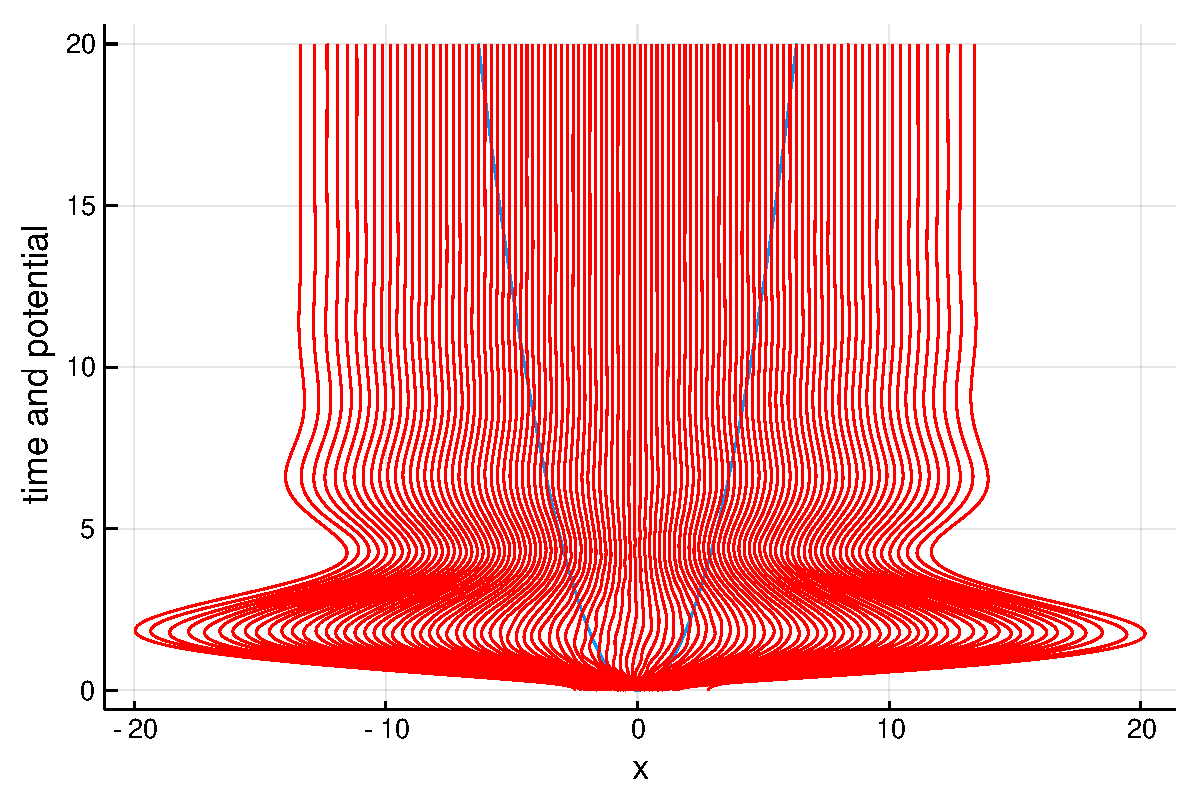
\includegraphics[width=\linewidth]{figures/Lecture16_4_1.pdf}

As the number of charges becomes large, they spread off to infinity. In the case of $V(x) = x^2$,  we can renormalize by  dividing by $N$ so they stay bounded: $\mu_k = {\lambda_k \over \sqrt N}$.


\begin{lstlisting}
(*@\HLJLn{p}@*) (*@\HLJLoB{=}@*) (*@\HLJLnf{plot}@*)(*@\HLJLp{(}@*)(*@\HLJLn{xx}@*)(*@\HLJLp{,}@*) (*@\HLJLn{V}@*)(*@\HLJLoB{.}@*)(*@\HLJLp{(}@*)(*@\HLJLn{xx}@*)(*@\HLJLp{);}@*) (*@\HLJLn{legend}@*)(*@\HLJLoB{=}@*)(*@\HLJLkc{false}@*)(*@\HLJLp{,}@*) (*@\HLJLn{xlabel}@*)(*@\HLJLoB{=}@*)(*@\HLJLs{"{}x"{}}@*)(*@\HLJLp{,}@*) (*@\HLJLn{ylabel}@*)(*@\HLJLoB{=}@*)(*@\HLJLs{"{}time}@*) (*@\HLJLs{and}@*) (*@\HLJLs{potential"{}}@*)(*@\HLJLp{)}@*)
(*@\HLJLk{for}@*) (*@\HLJLn{j}@*) (*@\HLJLoB{=}@*) (*@\HLJLni{1}@*)(*@\HLJLoB{:}@*)(*@\HLJLn{N}@*)
    (*@\HLJLnf{plot!}@*)(*@\HLJLp{(}@*)(*@\HLJLn{getindex}@*)(*@\HLJLoB{.}@*)(*@\HLJLp{(}@*)(*@\HLJLn{\ensuremath{\lambda}v}@*)(*@\HLJLoB{.}@*)(*@\HLJLp{(}@*)(*@\HLJLn{tt}@*)(*@\HLJLp{)}@*)(*@\HLJLoB{./}@*)(*@\HLJLnf{sqrt}@*)(*@\HLJLp{(}@*)(*@\HLJLn{N}@*)(*@\HLJLp{),}@*)(*@\HLJLn{j}@*)(*@\HLJLp{),}@*) (*@\HLJLn{tt}@*)(*@\HLJLp{;}@*) (*@\HLJLn{color}@*)(*@\HLJLoB{=:}@*)(*@\HLJLn{red}@*)(*@\HLJLp{)}@*)
(*@\HLJLk{end}@*)
(*@\HLJLn{p}@*)
\end{lstlisting}

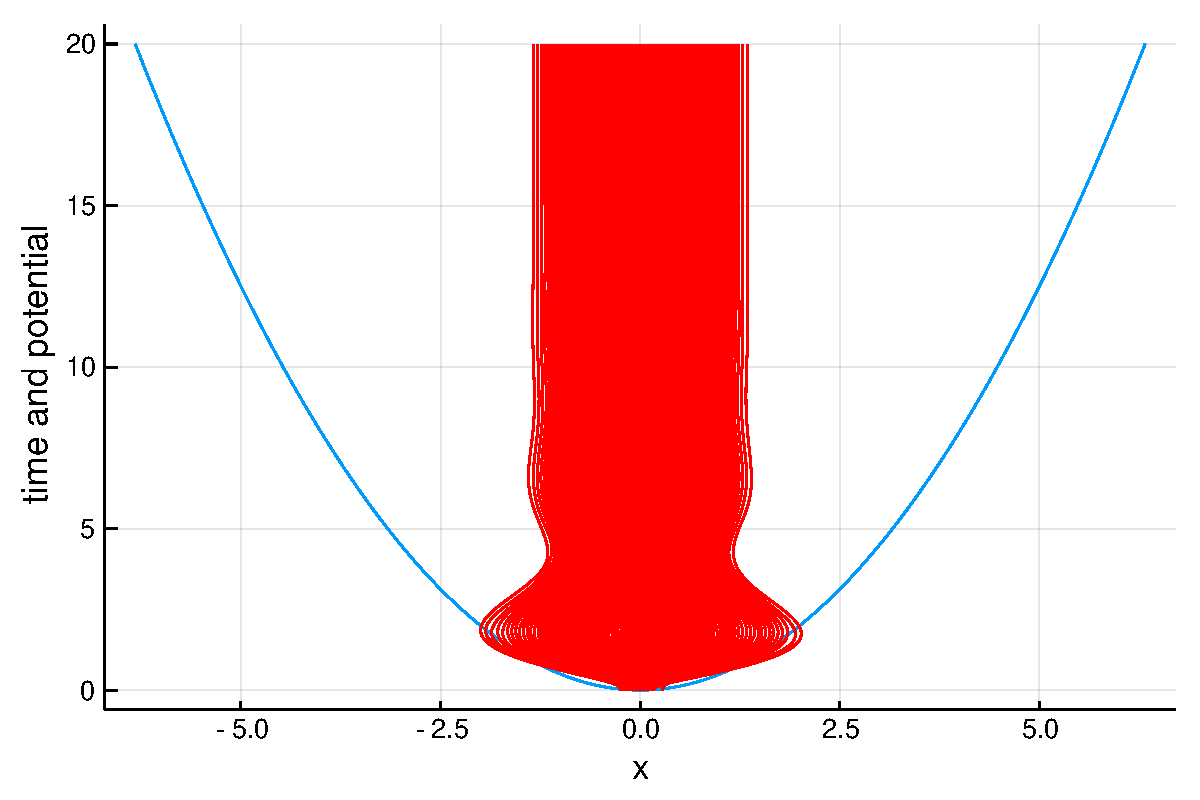
\includegraphics[width=\linewidth]{figures/Lecture16_5_1.pdf}

This begs questions: why does it balance out at $\pm \sqrt 2$?  Why does it have a nice histogram precisely like ${\sqrt{2-x^2} \over \pi}$:


\begin{lstlisting}
(*@\HLJLnf{histogram}@*)(*@\HLJLp{(}@*)(*@\HLJLn{\ensuremath{\lambda}v}@*)(*@\HLJLoB{.}@*)(*@\HLJLp{(}@*)(*@\HLJLnfB{20.0}@*)(*@\HLJLp{)[}@*)(*@\HLJLni{1}@*)(*@\HLJLoB{:}@*)(*@\HLJLn{N}@*)(*@\HLJLp{]}@*)(*@\HLJLoB{./}@*)(*@\HLJLnf{sqrt}@*)(*@\HLJLp{(}@*)(*@\HLJLn{N}@*)(*@\HLJLp{);}@*) (*@\HLJLn{nbins}@*)(*@\HLJLoB{=}@*)(*@\HLJLni{20}@*)(*@\HLJLp{,}@*) (*@\HLJLn{normalize}@*)(*@\HLJLoB{=}@*)(*@\HLJLkc{true}@*)(*@\HLJLp{,}@*) (*@\HLJLn{label}@*)(*@\HLJLoB{=}@*)(*@\HLJLs{"{}histogram}@*) (*@\HLJLs{of}@*) (*@\HLJLs{charges"{}}@*)(*@\HLJLp{)}@*)
(*@\HLJLnf{plot!}@*)(*@\HLJLp{(}@*)(*@\HLJLn{x}@*) (*@\HLJLoB{->}@*) (*@\HLJLnf{sqrt}@*)(*@\HLJLp{(}@*)(*@\HLJLni{2}@*)(*@\HLJLoB{-}@*)(*@\HLJLn{x}@*)(*@\HLJLoB{{\textasciicircum}}@*)(*@\HLJLni{2}@*)(*@\HLJLp{)}@*)(*@\HLJLoB{/}@*)(*@\HLJLp{(}@*)(*@\HLJLn{\ensuremath{\pi}}@*)(*@\HLJLp{),}@*) (*@\HLJLnf{range}@*)(*@\HLJLp{(}@*)(*@\HLJLnf{eps}@*)(*@\HLJLp{()}@*)(*@\HLJLoB{-}@*)(*@\HLJLnf{sqrt}@*)(*@\HLJLp{(}@*)(*@\HLJLnfB{2.0}@*)(*@\HLJLp{);}@*) (*@\HLJLn{stop}@*)(*@\HLJLoB{=}@*)(*@\HLJLnf{sqrt}@*)(*@\HLJLp{(}@*)(*@\HLJLni{2}@*)(*@\HLJLp{)}@*)(*@\HLJLoB{-}@*)(*@\HLJLnf{eps}@*)(*@\HLJLp{(),}@*) (*@\HLJLn{length}@*)(*@\HLJLoB{=}@*)(*@\HLJLni{100}@*)(*@\HLJLp{),}@*) (*@\HLJLn{label}@*)(*@\HLJLoB{=}@*)(*@\HLJLs{"{}semicircle"{}}@*)(*@\HLJLp{)}@*)
\end{lstlisting}

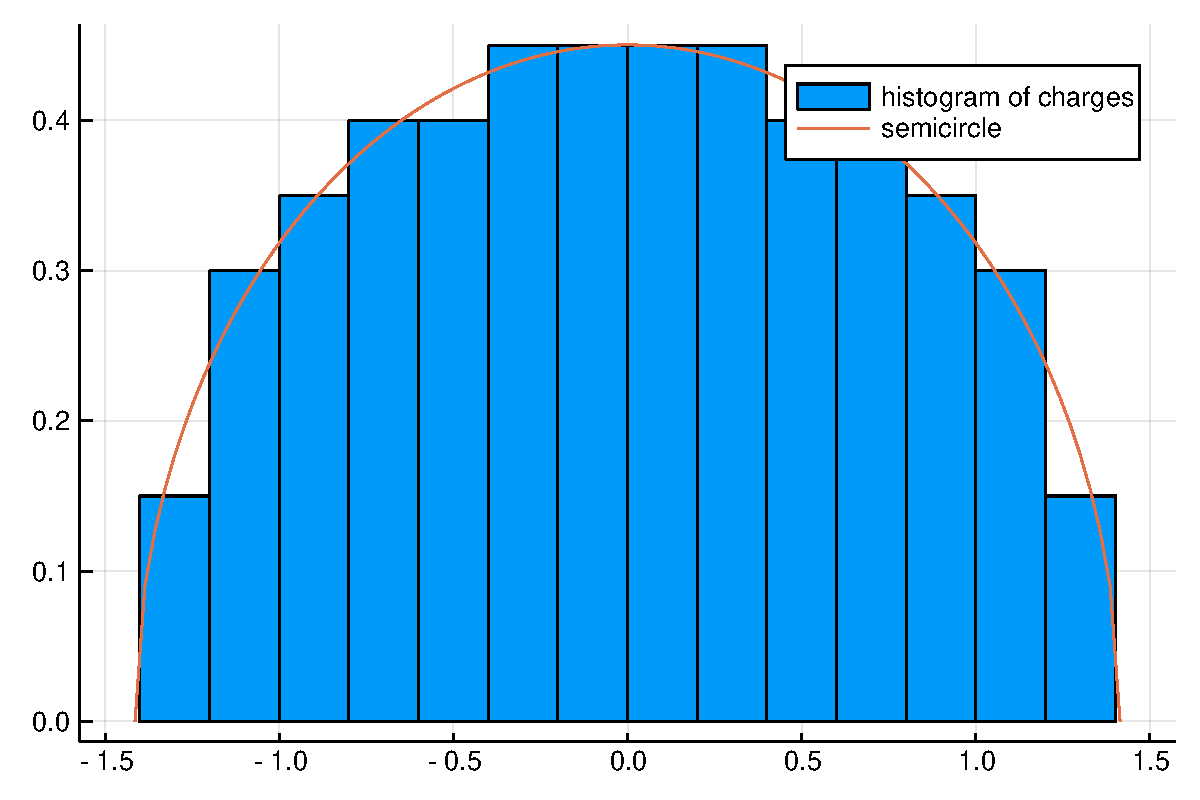
\includegraphics[width=\linewidth]{figures/Lecture16_6_1.pdf}

\subsubsection{Equilibrium distribution}
Plugging in $\lambda_k = \sqrt N \mu_k$, we get a dynamical system for $\mu_k$:

\[
 m {\D^2  \mu_k \over \D t} + \gamma {\D  \mu_k \over \D t}= {1 \over N} \sum_{j=1 \atop j \neq k}^N {1 \over \mu_k -\mu_j} -  \mu_k
\]
(The choice of scaling like $\sqrt N$ was dictated by $V'(x)$, if $V(x) = x^4$ it would be $N^{1/4}$.)  Thus the limit of the charges is given when the change with $t$ vanishes, that is 

\[
0 = {1 \over N} \sum_{j=1 \atop j \neq k}^N {1 \over \mu_k -\mu_j} -  \mu_k 
\]
It is convenient to represent the point charges by Dirac delta functions:

\[
    w_N(x) = {1 \over N} \sum_{k=1}^N \delta_{\mu_k}(x)
\]
normalized so that $\int w_N(x) \dx = 1$, so that

\[
    {1 \over N} \sum_{k=1}^N {1 \over  x -\mu_j} = \int_{-\infty}^\infty {w_N(t) \dt \over x - t}
\]
or in other words, we have 

\[
 \HH_{(-\infty,\infty)} w_N(\mu_k) = {V'(\mu_k) \over \pi}
\]
since

\[
\HH w_n (\mu_k) = {1 \over \pi} \lim_{\epsilon\rightarrow 0} \left(\int_{-\infty}^{\mu_k-\epsilon} + \int_{\mu_k+\epsilon}^\infty\right) {w_N(t)  \over  \mu_k-t} \dt  = {1 \over N\pi} \sum_{j \neq k} {1 \over \mu_k - \mu_j}
\]
Formally (see a more detailed explanation below), $w_N(x)$ tends to a continuous limit as $N\rightarrow \infty$,  which we have guessed from the histogram to be $w(x) = { \sqrt{2-x^2}  \over \pi}$ for $-\sqrt 2 < x < \sqrt2$.   We expect this limit to satisfy the same equation as $w_n$, that is

\[
 \HH w(x) = {x \over \pi}
\]
for $x$ in the support of $w(x)$.

Why is it $[-\sqrt 2, \sqrt 2]$? Consider the problem posed on a general interval $[a,b]$ where $a$ and $b$ are unknowns.  We  want to choose the interval $[a,b]$ so that there exists a $w(x)$  satisfying

\begin{itemize}
\item[1. ] \[
w
\]
is bounded (Based on observation)


\item[2. ] \[
w(x) \geq 0
\]
for $a \leq x \leq b$ (Since it is a probability distribution)


\item[3. ] \[
\int_a^b w(x) \dx = 1
\]
(Since it is a probability distribution)


\item[4. ] \[
\HH_{[a,b]} w(x) = x/\pi
\]
\end{itemize}
As we saw last lecture, there exists a bounded solution to  $\HH_{[-b,b]} u =  x/\pi$, namely  $u(x) = { \sqrt{b^2-x^2} \over \pi}$. The choice $b = \sqrt{2}$ ensures that $\int_{-b}^b u(x) \dx = 1$, hence $u(x) = w(x)$.

\subsubsection{Aside: Explanation of limit of $w_N(x)$}
This is beyond the scope of the course, but the convergence of $w_N(x)$ to $w(x)$ is known as weak-* convergence.  A simple version of this is that

\[
   \int_c^d w_N(x) \dx \rightarrow \int_c^d w(x) \dx
\]
for every choice of interval $(c,d)$. \$   {\textbackslash}int\emph{c\^{}d w}N(x) {\textbackslash}dx \$ is precisely the number of charges in  $(c,d)$ scaled by $1/N$,  which is exactly what a histogram plots.


\begin{lstlisting}
(*@\HLJLk{using}@*) (*@\HLJLn{ApproxFun}@*)(*@\HLJLp{,}@*) (*@\HLJLn{SingularIntegralEquations}@*)
(*@\HLJLn{a}@*) (*@\HLJLoB{=}@*) (*@\HLJLoB{-}@*)(*@\HLJLnfB{0.1}@*)(*@\HLJLp{;}@*) (*@\HLJLn{b}@*)(*@\HLJLoB{=}@*) (*@\HLJLnfB{0.3}@*)(*@\HLJLp{;}@*)
(*@\HLJLn{w}@*) (*@\HLJLoB{=}@*) (*@\HLJLnf{Fun}@*)(*@\HLJLp{(}@*)(*@\HLJLn{x}@*) (*@\HLJLoB{->}@*) (*@\HLJLnf{sqrt}@*)(*@\HLJLp{(}@*)(*@\HLJLni{2}@*)(*@\HLJLoB{-}@*)(*@\HLJLn{x}@*)(*@\HLJLoB{{\textasciicircum}}@*)(*@\HLJLni{2}@*)(*@\HLJLp{)}@*)(*@\HLJLoB{/}@*)(*@\HLJLn{\ensuremath{\pi}}@*)(*@\HLJLp{,}@*) (*@\HLJLn{a}@*) (*@\HLJLoB{..}@*) (*@\HLJLn{b}@*)(*@\HLJLp{)}@*)
(*@\HLJLnf{sum}@*)(*@\HLJLp{(}@*)(*@\HLJLn{w}@*)(*@\HLJLp{),}@*)  (*@\HLJLcs{{\#}}@*) (*@\HLJLcs{integral}@*) (*@\HLJLcs{of}@*) (*@\HLJLcs{w(x)}@*) (*@\HLJLcs{between}@*) (*@\HLJLcs{a}@*) (*@\HLJLcs{and}@*) (*@\HLJLcs{b}@*)
(*@\HLJLnf{length}@*)(*@\HLJLp{(}@*)(*@\HLJLnf{filter}@*)(*@\HLJLp{(}@*)(*@\HLJLn{\ensuremath{\lambda}}@*) (*@\HLJLoB{->}@*) (*@\HLJLn{a}@*) (*@\HLJLoB{\ensuremath{\le}}@*) (*@\HLJLn{\ensuremath{\lambda}}@*) (*@\HLJLoB{\ensuremath{\le}}@*) (*@\HLJLn{b}@*)(*@\HLJLp{,}@*) (*@\HLJLnf{\ensuremath{\lambda}v}@*)(*@\HLJLp{(}@*)(*@\HLJLnfB{20.0}@*)(*@\HLJLp{)[}@*)(*@\HLJLni{1}@*)(*@\HLJLoB{:}@*)(*@\HLJLn{N}@*)(*@\HLJLp{]}@*)(*@\HLJLoB{/}@*)(*@\HLJLnf{sqrt}@*)(*@\HLJLp{(}@*)(*@\HLJLn{N}@*)(*@\HLJLp{)))}@*)(*@\HLJLoB{/}@*)(*@\HLJLn{N}@*) (*@\HLJLcs{{\#}}@*) (*@\HLJLcs{integral}@*) (*@\HLJLcs{of}@*) (*@\HLJLcs{w{\_}N(x)}@*) (*@\HLJLcs{between}@*) (*@\HLJLcs{a}@*) (*@\HLJLcs{and}@*) (*@\HLJLcs{b}@*)
\end{lstlisting}

\begin{lstlisting}
(0.1790059168895313, 0.18)
\end{lstlisting}


Another varient of describing weak-* convergence is that the Cauchy transforms converge,  that is, for $z$ on any  contour $\gamma$ surrounding $a$ and $b$ (now the support of $w$) we have

\[
\int_a^b {w_N(x) \over x - z} \dx \rightarrow \int_a^b {w(x) \over x - z} \dx
\]
converges uniformly with respect to $N \rightarrow \infty$. here we demonstrate it converges at a point:


\begin{lstlisting}
(*@\HLJLn{x}@*) (*@\HLJLoB{=}@*) (*@\HLJLnf{Fun}@*)(*@\HLJLp{(}@*)(*@\HLJLoB{-}@*)(*@\HLJLnf{sqrt}@*)(*@\HLJLp{(}@*)(*@\HLJLni{2}@*)(*@\HLJLp{)}@*) (*@\HLJLoB{..}@*) (*@\HLJLnf{sqrt}@*)(*@\HLJLp{(}@*)(*@\HLJLni{2}@*)(*@\HLJLp{))}@*)
(*@\HLJLn{w}@*) (*@\HLJLoB{=}@*) (*@\HLJLnf{sqrt}@*)(*@\HLJLp{(}@*)(*@\HLJLni{2}@*)(*@\HLJLoB{-}@*)(*@\HLJLn{x}@*)(*@\HLJLoB{{\textasciicircum}}@*)(*@\HLJLni{2}@*)(*@\HLJLp{)}@*)(*@\HLJLoB{/}@*)(*@\HLJLn{\ensuremath{\pi}}@*)
(*@\HLJLn{z}@*) (*@\HLJLoB{=}@*) (*@\HLJLnfB{0.1}@*)(*@\HLJLoB{+}@*)(*@\HLJLnfB{0.2}@*)(*@\HLJLn{im}@*)
(*@\HLJLnf{cauchy}@*)(*@\HLJLp{(}@*)(*@\HLJLn{w}@*)(*@\HLJLp{,}@*) (*@\HLJLn{z}@*)(*@\HLJLp{),}@*) (*@\HLJLp{(}@*)(*@\HLJLnf{sum}@*)(*@\HLJLp{(}@*)(*@\HLJLni{1}@*) (*@\HLJLoB{./}@*)(*@\HLJLp{((}@*)(*@\HLJLnf{\ensuremath{\lambda}v}@*)(*@\HLJLp{(}@*)(*@\HLJLnfB{10.0}@*)(*@\HLJLp{)[}@*)(*@\HLJLni{1}@*)(*@\HLJLoB{:}@*)(*@\HLJLn{N}@*)(*@\HLJLp{]}@*)(*@\HLJLoB{/}@*)(*@\HLJLnf{sqrt}@*)(*@\HLJLp{(}@*)(*@\HLJLn{N}@*)(*@\HLJLp{))}@*) (*@\HLJLoB{.-}@*) (*@\HLJLn{z}@*)(*@\HLJLp{))}@*)(*@\HLJLoB{/}@*)(*@\HLJLn{N}@*)(*@\HLJLp{)}@*)(*@\HLJLoB{/}@*)(*@\HLJLp{(}@*)(*@\HLJLni{2}@*)(*@\HLJLn{\ensuremath{\pi}}@*)(*@\HLJLoB{*}@*)(*@\HLJLn{im}@*)(*@\HLJLp{)}@*)
\end{lstlisting}

\begin{lstlisting}
(0.1949409042727309 + 0.013681505291622225im, 0.196209148881836 + 0.0138401
97242559325im)
\end{lstlisting}



\end{document}
